\documentclass[12pt, a4paper]{article}

%PACK------------------------------
\usepackage[utf8]{inputenc}
\usepackage[T1]{fontenc}
\usepackage[british, polish]{babel}
\usepackage{geometry}
\usepackage{gensymb} %pakiet symboli
%\usepackage[upgreek, LGRgreek]{mathastext}
\usepackage{upgreek}
\usepackage{bm}
\usepackage{lipsum}
\usepackage{cite}
\usepackage{graphicx}
\usepackage{hyperref}
\usepackage{seqsplit}
\usepackage[table, xcdraw]{xcolor}
\usepackage{mathptmx}
\usepackage{fontspec}
\usepackage{textcomp}
\usepackage{adjustbox}
\usepackage{amsmath}

%SETTING---------------------------
%\defaultfontfeatures{LetterSpace=5}
\setmainfont{Times New Roman}
\setlength{\parindent}{0pt}
\setlength{\parskip}{0pt}
\linespread{1.25}
\geometry{left=2.54cm, right=2.54cm, top=2.54cm, bottom=2.54cm}
% \renewcommand{\thesection}{\arabic{section}.}
% \renewcommand{\thesubsection}{\thesection\arabic{subsection}.}
\newcommand*{\myfont}{\fontfamily{pcr}\selectfont}

%DOCUMENT--------------------------
\begin{document}
\begin{titlepage}
    \thispagestyle{empty}
    \begin{center}
    
        \textbf{\large Uniwersytet Jagielloński w Krakowie}
        
        \vspace{0.5cm}
        
        \textbf{\Large Wydział Biochemii, Biofizyki i Biotechnologii}
        
        \vspace{0.5cm}
        
        \begin{figure}[h]
            \centering
            \includegraphics[width=4cm]{figures/Herb_Uniwersytetu_Jagiellońskiego.svg.png}
            \label{fig:title}
        \end{figure}
        
        \vspace{0.5cm}

        \textbf{\huge Optymalizacja pomiarów napięcia w~układzie MFC z jednoczesną produkcją MlrA w komórkach \textit{Synechocystis sp.}}

        \vspace{2cm}

        {\Large Filip Stanisław Hajdyła}\\
        Nr albumu: 1164936

        \vspace{2cm}
        
        {\large Praca licencjacka z Biotechnologii}
        
        \vspace{0.5cm}
        
        {\large pod opieką dr hab. Dariusza Dzigi}
        
        \vspace{1cm}
        
        \textbf{\Large Pracownia Metabolomiki}
        
        \vspace{2cm}
        
        Kraków, 2022
        
    \end{center}
\end{titlepage}

\newpage
\thispagestyle{empty}
\tableofcontents

\newpage
\thispagestyle{empty}
\vspace*{\fill}
\begin{abstract}
    \noindent
    \lipsum[1]
\end{abstract}

\vspace{0.5cm}

\begin{center}
    \rule{150pt}{0.4pt}
\end{center}

\vspace{0.5cm}

\begin{otherlanguage}{british}
    \begin{abstract}
        \noindent
        \lipsum[1]
    \end{abstract}
\end{otherlanguage}
\vspace*{\fill}

%\vspace*{3cm}
%\begin{flushright}
%    Dziękuję Panu Profesorowi Dariuszowi Dzidze\\
%    oraz pozostałym członkom Pracowni Metabolomiki\\
%    za cierpliwość, wyrozumiałość, cenne rady\\
%    oraz pomoc w realizacji eksperymentów.
%\end{flushright}
%\vspace*{\fill}
%\begin{flushleft}
%    \textit{Non omnis moriar!}
%\end{flushleft}

\newpage
\setcounter{page}{4}
\section{Wstęp}\label{sec:wstep}
\subsection{Historia \acrshort{mfc}}\label{subsec:historia}
\acrshort{mfc} (\textit{ang.} \acrlong{mfc}) to urządzenia umożliwiające
generowanie energii elektrycznej z wykorzystaniem mikroorganizmów.
Należą one do szerszej klasy urządzeń \acrshort{bes} (\textit{ang.}
\acrlong{bes})~\cite{Santoro2017}.
Pomysł wykorzystania mikroorganizmów do generowania elektryczności
przypisuje się Michaelowi Potterowi~\cite{Potter1911},
natomiast idea ,,elektryczności zwierząt'', a więc elektryczności
związanej z układami ożywionymi, sięga aż XVIII wieku~\cite{Santoro2017}.
Pomimo iż pracę Pottera uważa się za początek technologii \acrshort{mfc},
dopiero po ponad 50 latach od jej publikacji
znalazła ona praktyczne zastosowanie w oczyszczaniu i przetwarzaniu
odpadów ściekowych w prąd elektryczny podczas lotów kosmicznych
organizowanych przez \acrshort{nasa}~\cite{Slate2019}.

\subsection{Zastosowania \acrshort{mfc}}\label{subsec:zastosowania-mfc}

\begin{figure}[!b]
    \centering
    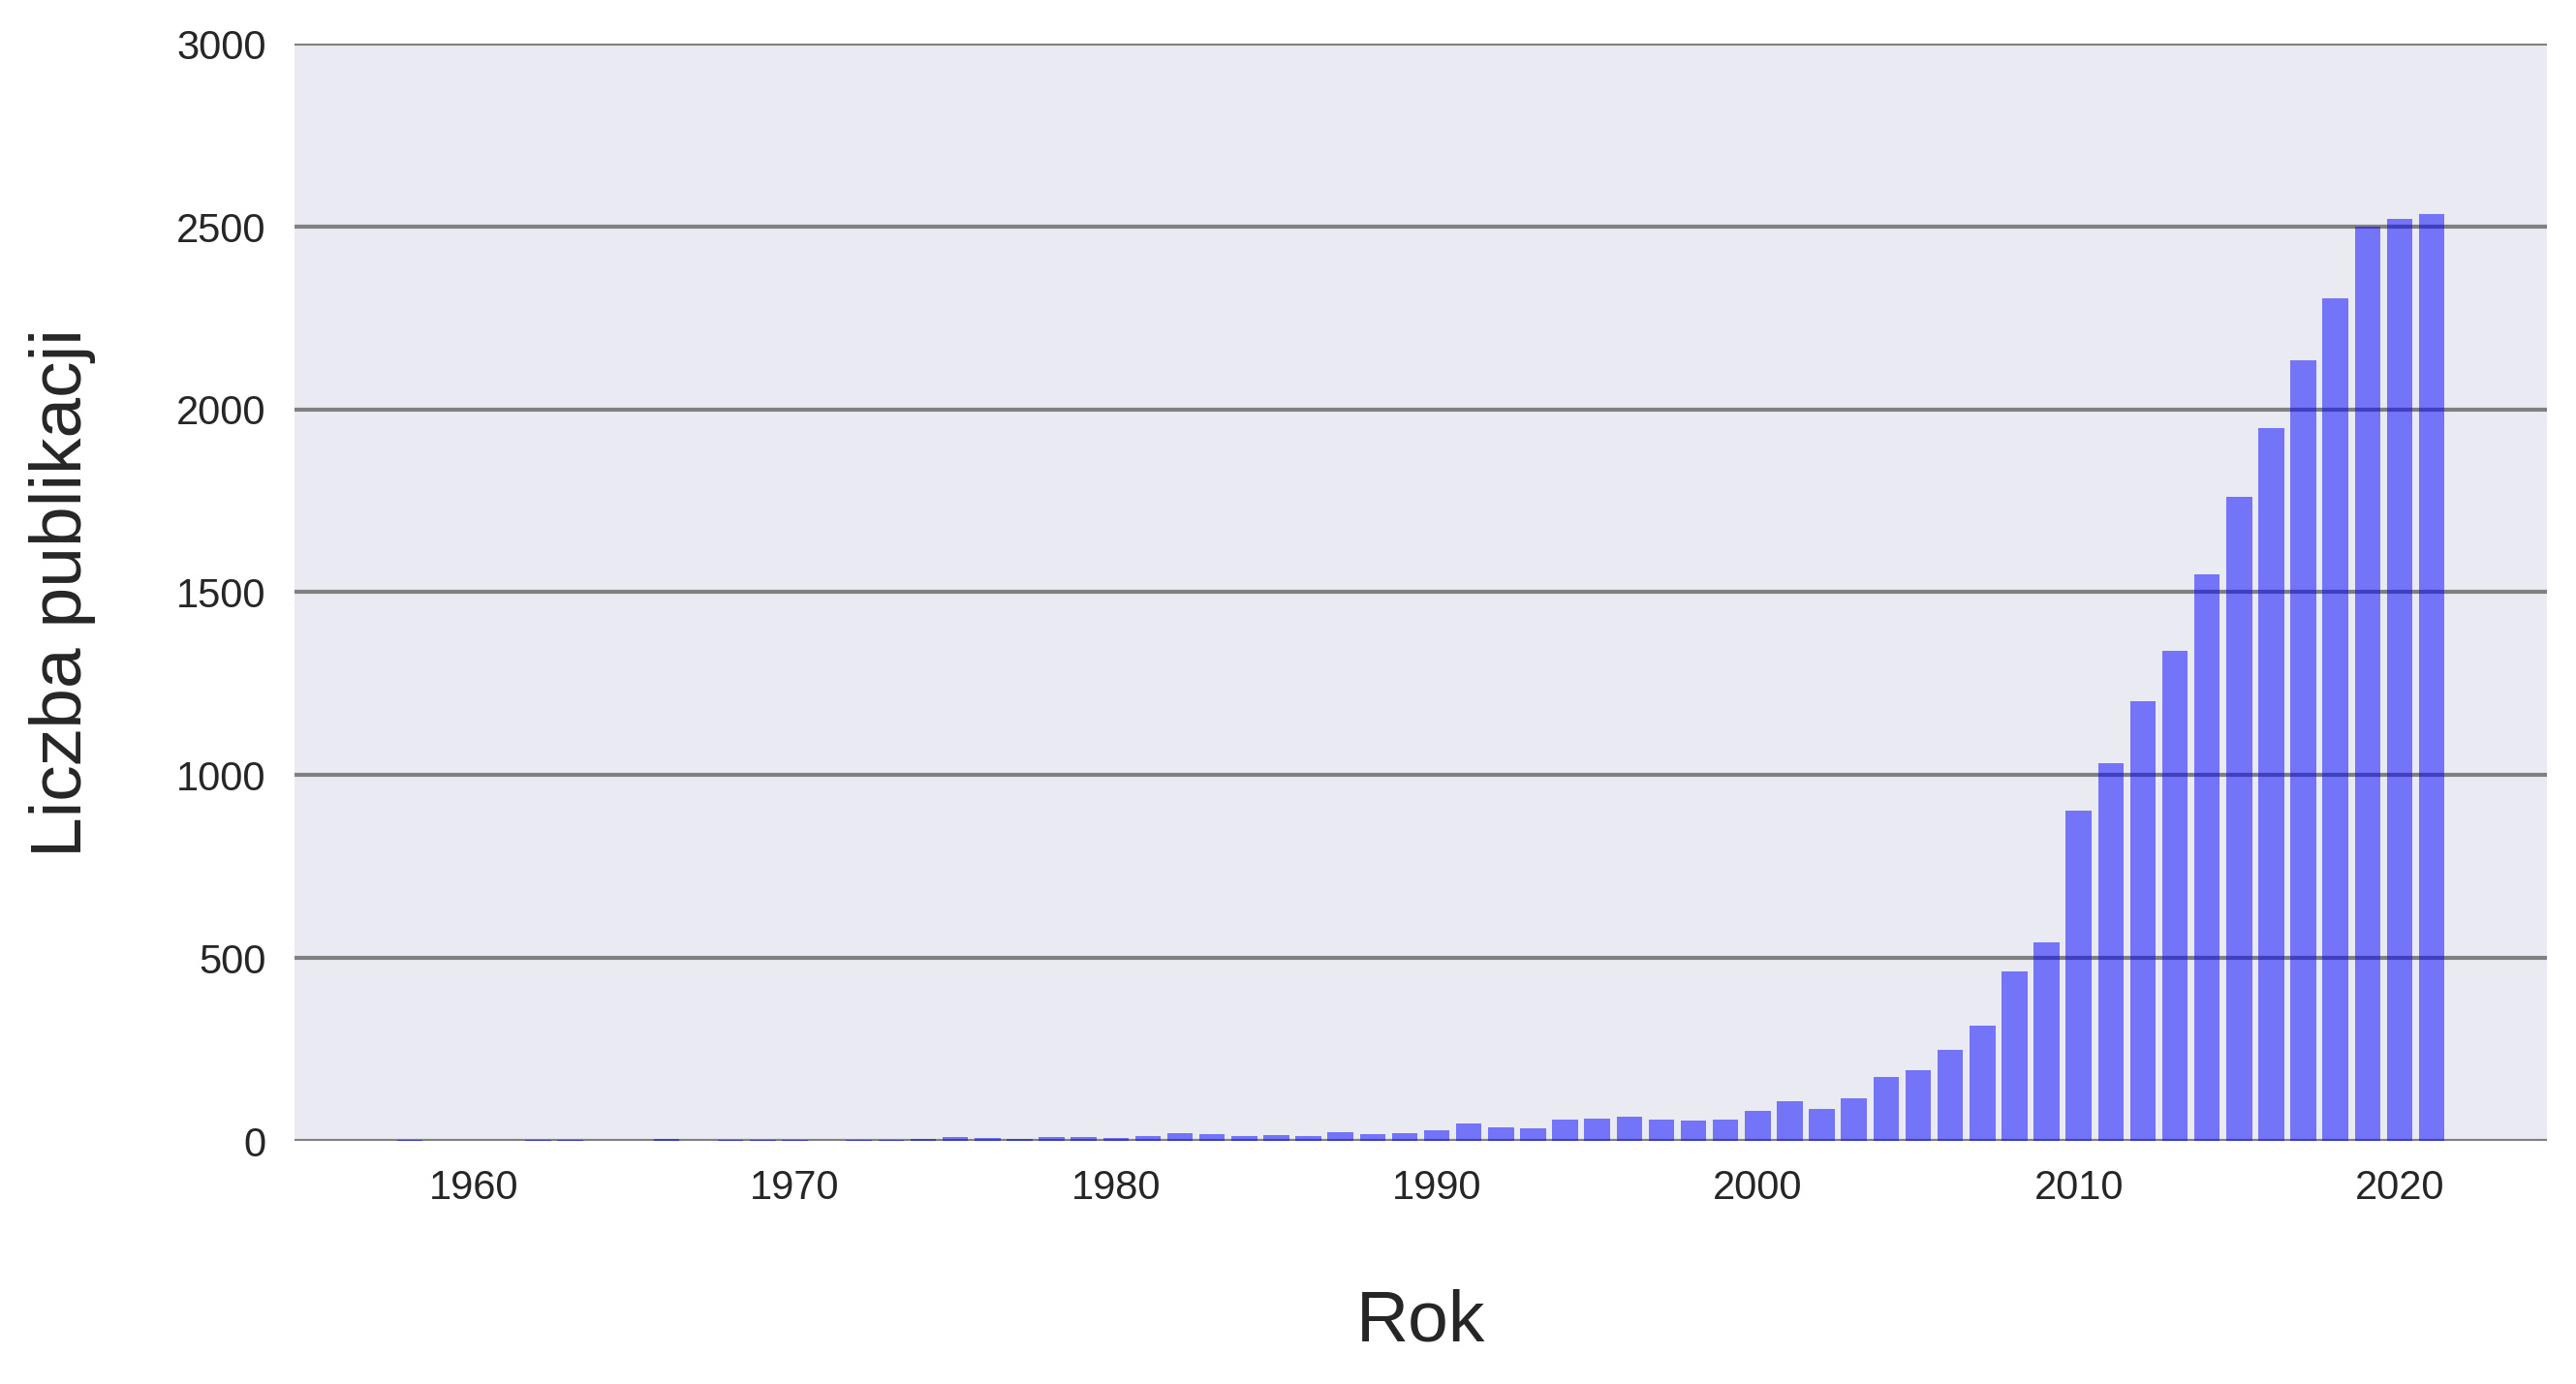
\includegraphics[width=12cm]{figures/publications}
    \caption{
        Liczba publikacji z ,,\acrshort{mfc}'' lub
        ,,\acrlong{mfc}'' w tytule w latach 1958--2021.
        (Dane pochodzą z serwisu \url{https://webofscience.com})
    }
    \label{fig:1}
\end{figure}

W ostatniej dekadzie zainteresowanie systemami \acrshort{bes},
a w szczególności \acrshort{mfc}, wzrosło diametralnie, co odzwierciedla wzrost
liczby związanych z nimi publikacji przedstawiony na rys.~\ref{fig:1}.
Pojawiające się publikacje związane z \acrshort{mfc}
dotyczą różnych aspektów tej technologii.
Wiele z nich dotyczy zrozumienia molekularnych podstaw
działania tych systemów~\cite{Slate2019, Bruce2006, Lovley2006}, inne
poruszają kwestie związane z ich konstrukcją i użyciem odpowiednich
materiałów do budowy elektrod i membran~\cite{Kaur2020, Daud2015},
a jeszcze inne skupiają się na bardzo istotnych
aspektach ekonomicznych~\cite{Trapero2017}.
Wysokie zainteresowanie technologią \acrshort{mfc} w ostatnich latach wynika
z potencjału do wykorzystania ich w celu jednoczesnego oczyszczania
wód ściekowych, generowania energii elektrycznej oraz produkcji cennej biomasy,
która mogłaby następnie zostać wykorzystana w biorafineriach do produkcji
biopaliw, biopolimerów i biochemikaliów.
Niewątpliwymi zaletami tych systemów są również ich długi czas działania
bez konieczności konserwacji i obsługi~\cite{Habermann1991}
oraz niewymagające warunki operacyjne~\cite{Slate2019}.
Obecne systemy oczyszczania ścieków wykorzystujące osad czynny
zużywają od 0.3 do 0.6 kWh m\textsuperscript{-3} co w skali globalnej
przekłada się na 4 \% całkowitego zużycia energii~\cite{AlSayed2020}.
Wszystkie ww.\ zalety systemów \acrshort{mfc} sprawiają natomiast, że mogłyby one
być częściowym rozwiązaniem problemu nadmiernej akumulacji odpadów,
umożliwiając ich energetycznie korzystną biokonwersję.
Obecnie uważa się, że systemy te nie są w stanie całkowicie zastąpić
tradycyjnych oczyszczalni ścieków, ale mogłyby służyć
jako jeden z komponentów nowoczesnych oczyszczalni połączonych
z biorafineriami.

\subsection{Podstawy molekularne działania \acrshort{amfc}}\label{subsec:podstawy-molekularne}
W systemach \acrshort{amfc} (\acrlong{amfc}), do generowania elektryczności, wykorzystuje się
utleniająco-redukujący charakter reakcji metabolicznych
przeprowadzanych przez mikroorganizmy, które możemy podzielić
na rezydujące na powierzchni anody elektrogeny (uwalniające na nią
elektrony) oraz zasiedlające katodę elektrotrofy
(pobierające i wykorzystujące elektrony)~\cite{AlSayed2020}.
Elektrogeny przeprowadzają procesy oddychania beztlenowego,
utleniając znajdujące się w pożywce związki organiczne oraz
wykorzystując anodę jako ostateczny akceptor elektronów.
Przykładem takiego procesu może być utlenianie octanu:
\begin{equation}
    \label{eq:1}
    \mathrm{CH_3 COO^- + 4H_2 O \rightarrow 2HCO_3^- + 9H^+ + 8e^-}
\end{equation}
Zdolność do transferu elektronów na powierzchnię metali (lub
innych przewodników) wynika z~naturalnego przystosowania tych
organizmów do życia na powierzchni rud metali i wykorzystania
ich jako ostateczny akceptor elektronów.
Transfer elektronów na elektrodę może zachodzić na różne
sposoby~\cite{Santoro2017}:

\begin{enumerate}
    \item Transport bezpośredni (z wykorzystaniem cytochromu c);
    \item Transport przez nano-przewody;
    \item Transport za pośrednictwem mediatorów redox;
\end{enumerate}

Choć nie poznano jeszcze dokładnie molekularnych mechanizmów
transferu elektronów, wiadomo, że najwolniejszym oraz
niekorzystnym z technologicznego punktu widzenia sposobem jest
transport za pośrednictwem mediatorów redox, gdyż jest on znacznie
ograniczony szybkością dyfuzji.
Do najbardziej efektywnych elektrogenów należą
\textit{Geobacter sulfurreducens}, \textit{Shwanella oneidensis}
oraz \textit{Rhodobacter sphaeroides}.
Elektrotrofy są z kolei organizmami pobierającymi elektrony
z powierzchni katody (za pośrednictwem mediatorów redox)
i redukującymi CO\textsubscript{2}, lub organizmami przeprowadzającymi fotosyntezę
oksygeniczną~\cite{Santoro2017, Reddy2019}.
Uwolniony w wyniku procesu fotosyntezy tlen jest następnie wykorzystywany
do utylizacji elektronów w reakcji redukcji tlenu do wody:
\begin{equation}
    \label{eq:2}
    \mathrm{O_2 + 2H^+ + 2e^- \rightarrow H_2 O}
\end{equation}
Użycie organizmów zapewniających wysokie tempo zużycia elektronów np.
intensywnie fotosyntetyzujących alg, takich jak \textit{Chlorella vulgaris},
lub cyjanobakterii z rodzaju \textit{Synechocystis} pozwala na efektywne
zapewnienie odpowiednich ilości tlenu w komorze katodowej bez
konieczności jej mechanicznego napowietrzania, co pozwala dodatkowo
zmniejszyć koszty operacyjne~\cite{Reddy2019}.
Należy jednak pamiętać, aby zapewnić odpowiednie warunki
organizmom bytującym w komorze z katodą.

\subsection{Cel pracy}\label{subsec:badania}
W niniejszej pracy przeprowadzono wstępne badania wzrostu organizmów
elektrogenicznych i elektrotroficznych
w środowisku o wysokim zanieczyszczeniu związkami
organicznymi, z jednoczesnym pomiarem aktywności mikrocystynazy
\acrshort{mlra}~\cite{Dexter2018, Dexter2021} w komórkach elektrotrofów
(\textit{Synechocystis sp.} PCC 6803),
oraz na optymalizacji pomiarów napięcia prądu elektrycznego generowanego
podczas wzrostu i metabolizmu tych mikroorganizmów.
Praca Pani Konstancji Gałat dowiodła, że w przypadku
hodowli z użyciem rozcieńczonych ścieków komunalnych (\acrshort{ww})
jako pożywki, największą ekspresję \acrshort{mlra} wykazuje szczep
\textit{Synechocystis sp.} PCC 6803 McCormick 7 rosnący na pożywce
z dodatkiem \acrshort{ww}2 (\ref{subsec:odczynniki})~\cite{Galat2022},
dlatego w niżej opisanych badaniach użyty został właśnie ten szczep,
a do jego kultywacji wykorzystano ww.\ substrat.

\section{Materiały i metody}\label{sec:metody}
\subsection{Sprzęt i oprogramowanie}\label{subsec:sprzet}
Do pomiarów gęstości optycznej (\acrshort{od}) używane były czytniki mikropłytek
Molecular Devices SpectraMax iD5, BioRad iMark
Microplate Reader, oraz spektrofotometr Unicam Helios $\upbeta$.
Do analizy aktywności \acrshort{mlra} metodą \acrshort{hplc} wykorzystano chromatograf
Agilent Technologies 1220 Infinity LC\@.
W celu homogenizacji komórek używano homogenizatora
Bertin Technologies Precellys Evolution (8000 rpm, 4 cykle po 45 s)
oraz kuleczek szklanych.
Celem pomiaru i ustalania pH pożywek zastosowano pH-metr
BECKMAN $\Phi 50$ pH Meter.
Do budowy układu \acrshort{amfc} wykorzystano oprzyrządowanie
zakupione w Mirong Mirong Store (Chiny) z pojemnikami
o objętości 250 ml, membranę nafionową Sigma-Aldrich,
jako katodę -- płytkę mosiężną o powierzchni całkowitej 30
cm\textsuperscript{2}, jako anodę -- 3 płytki z włókna węglowego
o łącznej powierzchni całkowitej 84 cm\textsuperscript{2}
(warunki operacyjne układu:
$T =$ 20 \degree C, intensywność oświetlenia mierzona w miejscu
ustawienia butelek względem lampy była równa
70 $\upmu$mol fotonów m\textsuperscript{-2} s\textsuperscript{-1}).
Do pomiarów różnicy potencjałów pomiędzy elektrodami
w układzie \acrshort{amfc} użyto multimetru PeakTech 4000 wraz
z~dedykowanym oprogramowaniem do zbierania danych przy pomocy komputera.
Do analizy danych i wizualizacji wykorzystano oprogramowanie
MS Excel, OriginLabs oraz język programowania Python
(głównie moduły pandas i matplotlib).

\subsection{Odczynniki chemiczne}\label{subsec:odczynniki}
Media hodowlane BG-11 i M27 do hodowli \textit{Rhodobacter} oraz
wszystkie potrzebne bufory wykonywane były zgodnie ze standardowymi
protokołami dostępnymi w Pracowni Metabolomiki.
Mikrocystynazę-LR pochodzi ze szczepu \textit{Microcystis aeruginosa} PCC 6803
pozyskanego z Instytutu Pasteura (Paryż, Francja).
Ścieki komunalne (\acrshort{ww}) pochodzą z oczyszczalni ścieków w Myślenicach.
Są one ponumerowane wg.\ schematu 1 w dodatku.
Pozostałe odczynniki chemiczne zostały zakupione
w Merck Millipore (Burlington, MA, USA).
%Kwas trifluorooctowy (TFA), odczynnik Bradforda, bufor fosforanowy (pH 7),
%media, wody ściekowe (\acrshort{ww}) pochodzące z oczyszczalni w Myślenicach
%(numeracja objaśniona w dodatku -- tab.\ 1).
%(ta sekcja jeszcze nie jest gotowa)

\subsection{Wykorzystane szczepy}\label{subsec:szczepy}
\textit{Synechocystis sp.} PCC 6803 McCormick 7~\cite{Puchalski2021}
był kultywowany z użyciem standardowego medium BG-11 z~dodatkiem 50
$\upmu$l ml\textsuperscript{-1} kanamycyny, w kolbach Erlenmayera,
w temperaturze 28 \degree C i natężeniu światła
40 $\upmu$mol fotonów m\textsuperscript{-2} s\textsuperscript{-1}.
Kolby były umieszczone na wytrząsarce orbitalnej (110 rpm).
\textit{Rhodobacter sphaeroides} kultywowano na pożywce \acrshort{m27}
do hodowli \textit{Rhodobacter} przygotowanej wg.\ protokołu
dostępnego w~Pracowni Metabolomiki, w probówkach typu
Falcon (50 ml), w temperaturze 20 \degree C i natężeniu światła
40 $\upmu$mol fotonów m\textsuperscript{-2} s\textsuperscript{-1}.

\subsection{Badanie wzrostu \textit{R. sphaeroides} w pożywce z dodatkiem ścieków komunalnych}\label{subsec:rhodobacter}
W tym eksperymencie badano wzrost \textit{R. sphaeroides} przy
różnych rodzajach i rozcieńczeniach wód ściekowych w pożywce.
Eksperyment wykonano w dwóch turach.
W pierwszej turze, w~probówkach Falcon 15 ml sporządzono
mieszaniny pożywki \acrshort{m27} z~wodami ściekowymi nr 2, 3 i~4,
w~stężeniach 5 \%, 15 \% i~45~\% ($V$~=~14~ml).
Ustalono pH mieszanin do ok.\ 7.
Jako kontroli użyto pożywki \acrshort{m27} (pH 6.8).
Wszystkie próbki zaszczepiono 1 ml pierwotnej hodowli
\textit{R. sphaeroides}.
Pomiary \acrshort{od}\textsubscript{600} były wykonywane przy pomocy
spektrofotometru Unicam Helios $\upbeta$.
Drugą turę eksperymentu przygotowano w~sposób analogiczny.
Różnicą było testowanie innych stężeń wód ściekowych
(15~\%, 45 \% i~80 \%).
Hodowle wykonano w trzech powtórzeniach biologicznych.
Mierzono \acrshort{od}\textsubscript{595} przy pomocy czytnika
mikropłytek BioRad iMark Microplate Reader
(droga optyczna $l$ odpowiada 200 $\upmu$l roztworu w studzience).

\subsection{Badanie aktywności \acrshort{mlra} w \textit{Synechocystis sp.} PCC 6803 McCormick~7}\label{subsec:mlra}
Aktywność \acrshort{mlra} w komórkach
\textit{Synechocystis sp.} PCC 6803 McCormick 7 mierzono przy
różnych rodzajach \acrshort{ww} w pożywce.
W tym celu przygotowano mieszaniny BG-11 z \acrshort{ww}2 i \acrshort{ww}3
w proporcjach 1:1 w objętościach po 40 ml.
Kontrolą była pożywka BG-11.
Obliczono, że mając hodowlę macierzystą
o \acrshort{od}\textsubscript{600} = 0.746, w celu osiągnięcia
początkowego \acrshort{od}\textsubscript{600} = 0.200, należy zawiesić
komórki z odwirowanych (10733 RCF, 10 min) 10,72 ml hodowli
pierwotnej w 40 ml nowej pożywki.
Hodowle wykonano w trzech powtórzeniach biologicznych.
Markerem selekcyjnym była kanamycyna ($c$ = 50 $\upmu$g ml\textsuperscript{-1}).
Zbierano próbki hodowli po 1 ml w 4, 7, 10 i~14 dniu eksperymentu
i komórki zamrażano (-20 \degree C).
Po rozmrożeniu próbki homogenizowano (\ref{subsec:sprzet}),
a~następnie odwirowywano (16873 RCF, 5 min), a nadsącz
zbierano do nowych probówek typu Eppendorf 1.5 ml.
Na płytce 96-dołkowej przeprowadzono test aktywności \acrshort{mlra}\@.
Do studzienek dodano po 45 $\upmu$l mikrocystyny (1.5 mg ml\textsuperscript{-1})
i 5 $\upmu$l odpowiedniego, wcześniej zebranego nadsączu (lizatu)
w różnych rozcieńczeniach (1x i 10x).
Reakcję prowadzono przez 1 h, po czym zatrzymano ją
poprzez dodanie 5 $\upmu$l 1 \% \acrshort{tfa}\@.
Rozdział mieszaniny prowadzono przy pomocy techniki \acrshort{hplc} (\ref{subsec:sprzet}).
Celem normalizacji obliczonych na podstawie danych z \acrshort{hplc} aktywności białka
mierzono całkowite stężenie białka metodą Bradforda w 3 rozcieńczeniach:
\textbf{a} 5 $\upmu$l lizatu + 95 $\upmu$l buforu fosforanowego pH 7.0
+~100 $\upmu$l odczynnika Bradforda; \textbf{b} 2 $\upmu$l lizatu
+ 98 $\upmu$l buforu fosforanowego pH 7.0 +~100 $\upmu$l odczynnika;
\textbf{c} 1 $\upmu$l lizatu + 99 $\upmu$l buforu fosforanowego pH 7.0 +~100
$\upmu$l odczynnika.

\subsection{Pomiary napięcia w układzie \acrshort{mfc}}\label{subsec:volt}
W tym eksperymencie badano wpływ gęstości hodowli
\textit{R. sphaeroides} w komorze z anodą na generowane
w układzie \acrshort{mfc} napięcie.
W komorze z katodą znajdowały się komórki
\textit{Synechocystis sp.} PCC 6803 McCormick 7
zawieszone w 250 ml BG-11 + 50 \% \acrshort{ww}2
(\acrshort{od}\textsubscript{600} = 1.000).
Początkowo w komorze z anodą znajdowało się 250 ml
pożywki \acrshort{m27}, jednak na samej elektrodzie był
obecny wcześniej zaadaptowany biofilm \textit{R. sphaeroides}.
Dodawano po 1 ml stężonej zawiesiny \textit{R. sphaeroides}
i, po zmieszaniu, mierzono \acrshort{od}\textsubscript{600} oraz
zmiany napięcia prądu stałego (DC) przez ok.\ 200 min od
momentu dodania kolejnej porcji zawiesiny komórek.
Dla \acrshort{od}\textsubscript{600} = 0.743 pomiary prowadzono
przez ok.\ 160 min ze względu na awarię sprzętu, co podczas
analizy statystycznej (\ref{sec:wyniki}) przełożyło się
na mniejszą liczbę powtórzeń (n).

\section{Wyniki}\label{sec:wyniki}
Na rys.~\ref{fig:2} przedstawiono wyniki
eksperymentu~\ref{subsec:rhodobacter}.
W 10 dniu eksperymentu widoczny jest istotny
statystycznie spadek \acrshort{od}\textsubscript{600}
w próbkach o $c_{\acrshort{ww}} = 80$ \% względem próbek
o niższych stężeniach.
Oznacza to hamowanie wzrostu \textit{R. sphaeroides}
przy stężeniach \acrshort{ww} 80 \%.
Z~tego względu w kolejnych eksperymentach kultywowano
\textit{R. sphaeroides} na \acrshort{m27} + 50 \% \acrshort{ww}\@.
Rys.~\ref{fig:3} przedstawia wyniki
eksperymentu~\ref{subsec:mlra}.
(\ldots)
Na rys.~\ref{fig:4} przedstawiono wyniki pomiarów
napięcia w eksperymencie~\ref{subsec:volt}.
Z wykresu wynika, że największe napięcia generowane
są w przypadku hodowli \textit{R. sphaeroides}
o \acrshort{od}\textsubscript{600} w zakresie od 0.200 do 0.535,
przy czym hodowle gęstsze, o~\acrshort{od}\textsubscript{600} bliskim
0.500 wykazują spadki napięcia po dłuższym czasie.

\begin{figure}[h!]
    \centering
    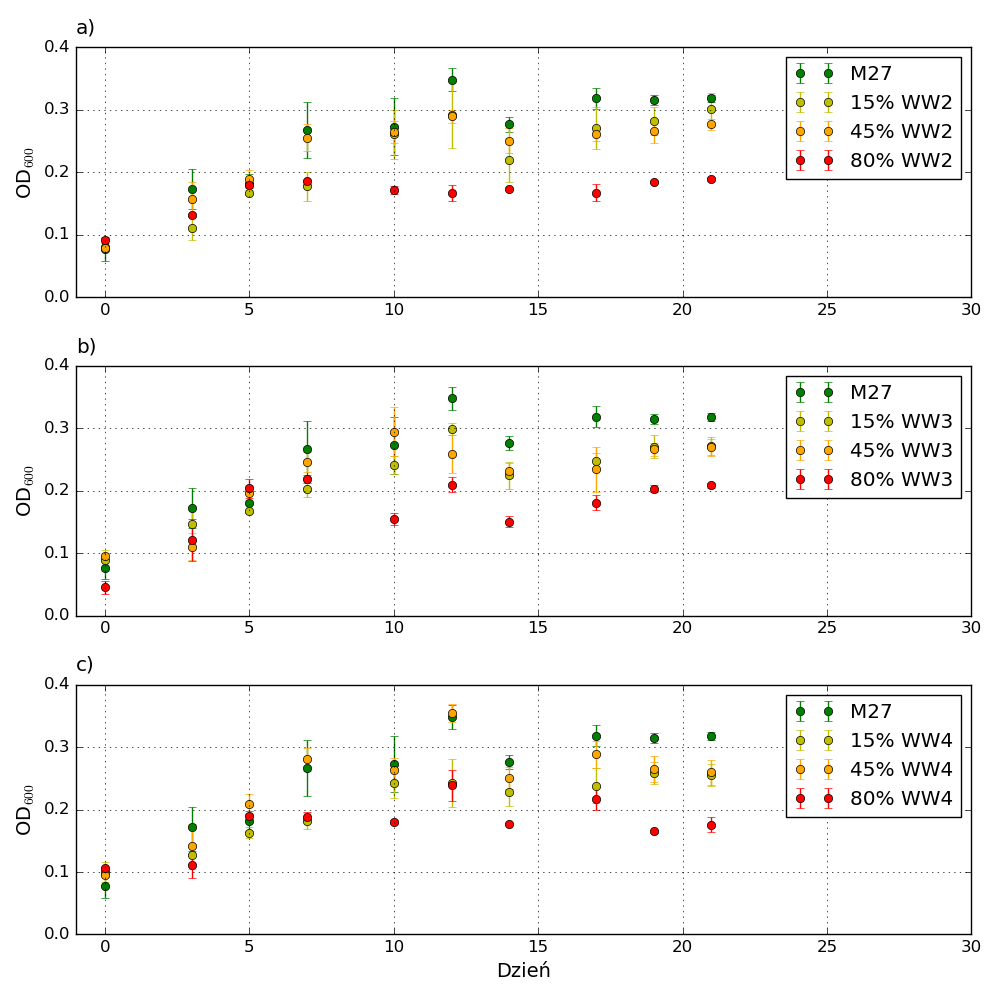
\includegraphics[width=13cm]{figures/ww}
    \caption{
        Zmiany \acrshort{od}\textsubscript{600} hodowli \textit{R. sphaeroides} w czasie w \acrshort{m27}:
        \textbf{a}~zawierającym \acrshort{ww}2 w~stężeniach 15 \%, 45 \% i 80 \%;
        \textbf{b}~zawierającym \acrshort{ww}3 w stężeniach 15 \%, 45 \% i 80 \%;
        \textbf{c}~zawierającym \acrshort{ww}4 w stężeniach 15 \%, 45 \% i 80 \%.
        Słupki błędów to \acrshort{sem} (n = 3).
    }
    \label{fig:2}
\end{figure}

\begin{figure}[h!]
    \centering
    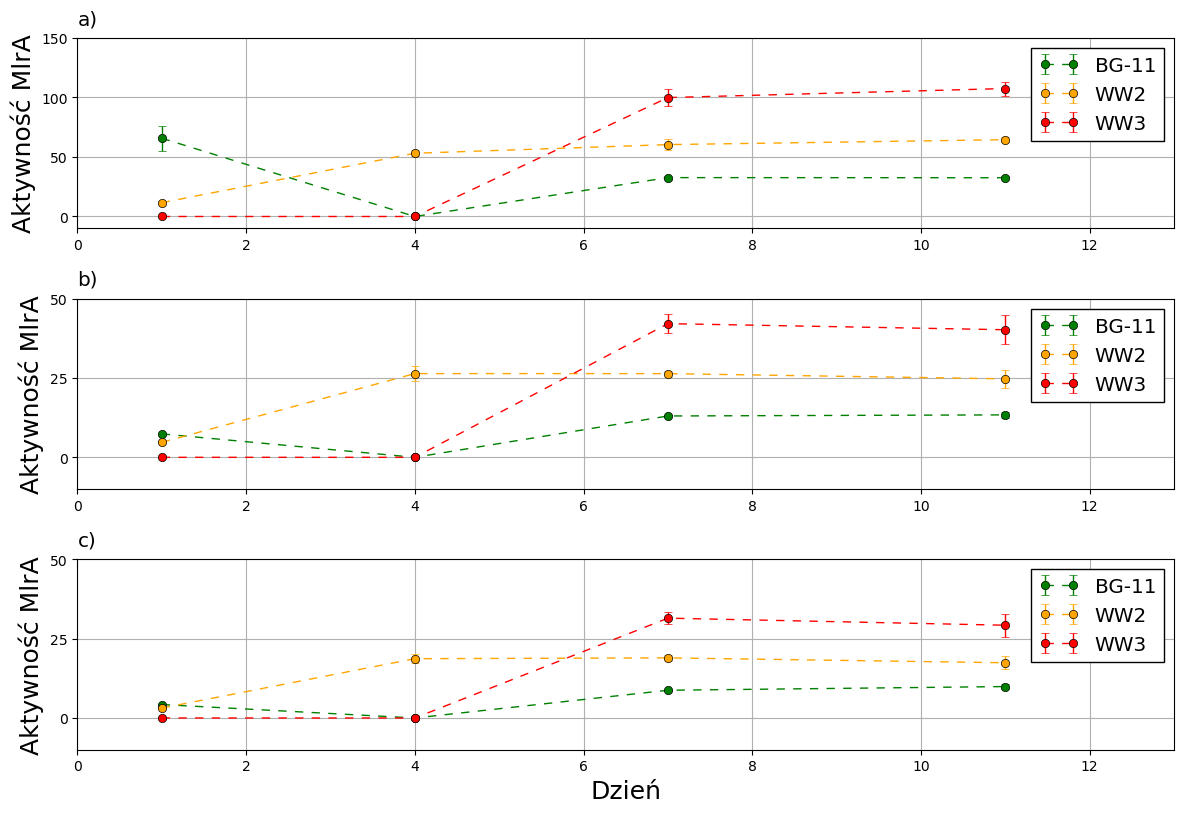
\includegraphics[width=13cm]{figures/mlra_activity}
    \caption{
        Aktywność \acrshort{mlra} w lizatach komórek
        \textit{Synechocystis sp.} PCC 6803 McCormick 7
        kultywowanych z użyciem różnych rodzajów \acrshort{ww} zmieszanych
        w proporcjach 1:1 z BG-11 jako pożywki. Słupki błędów to \acrshort{sem} (n = 3).
        Aktywność przeliczono na całkowitą zawartość białka w lizatach.
        Pomiar białka przeprowadzono w próbkach rozcieńczonych
        a) 20x; b) 50x; c) 100x.

    }
    \label{fig:3}
\end{figure}

\begin{figure}[h!]
    \centering
    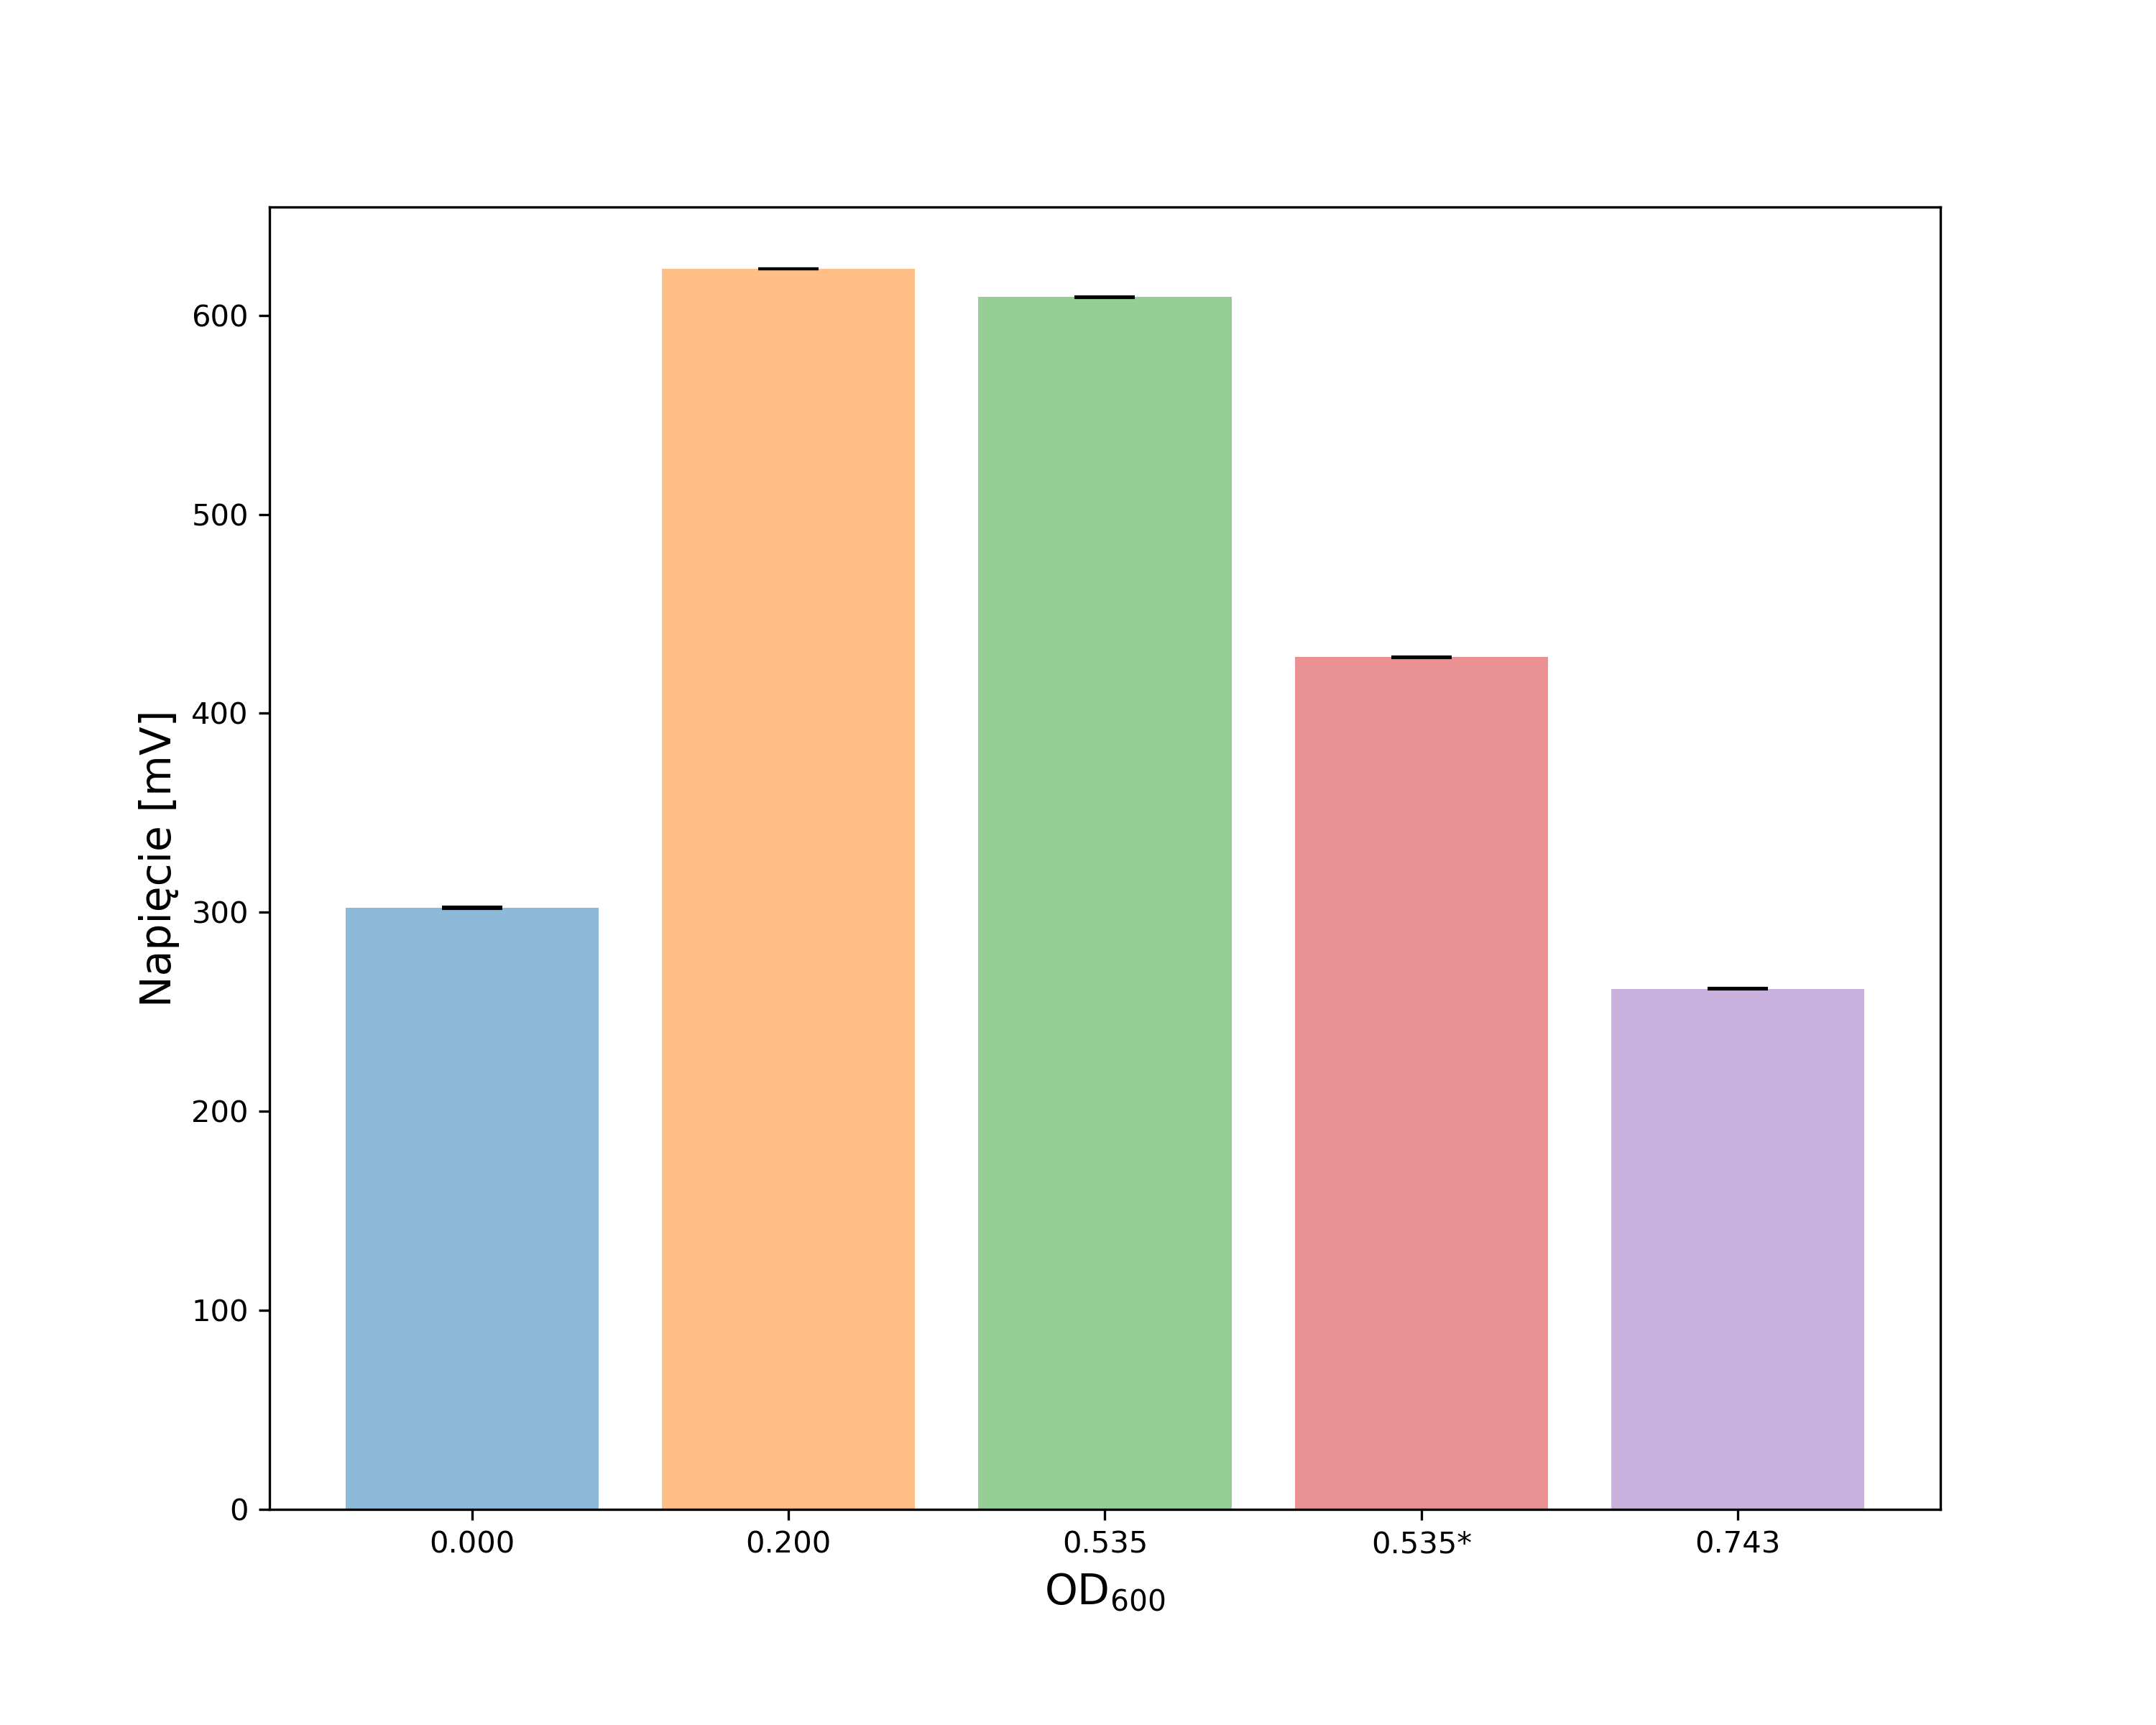
\includegraphics[width=12cm]{figures/voltage3}
    \caption{
        Uśrednione wartości napięcia w zależności od \acrshort{od}\textsubscript{600}
        hodowli \textit{R. sphaeroides} znajdującej się w komorze z anodą.
        *Pomiar wykonany po 24 h adaptacji mikroorganizmów do elektrody.
        Słupki błędów to \acrshort{sem} (n = 11; dla \acrshort{od}\textsubscript{600} = 0.743, n = 8).
    }
    \label{fig:4}
\end{figure}


\section{Wnioski}\label{sec:wnioski}
%RHODOBACTER
Wzrost \textit{R. sphaeroides}, badany poprzez pomiar
\acrshort{od}\textsubscript{600}, na pożywkach zawierających
\acrshort{ww} w~stężeniach nieprzekraczających 50~\%
nie został zahamowany w sposób istotny statystycznie.
Dopiero w przypadku 80~\% \acrshort{ww} wzrost był hamowany
po ok.\ 7-10 dniach hodowli.
Co ciekawe, nie było to zależne od rodzaju stosowanych
\acrshort{ww}, co wskazuje na niewrażliwość komórek
\textit{R.~sphaeroides} na różnego rodzaju zanieczyszczenia
i metabolity wtórne występujące w ściekach komunalnych
na różnych etapach oczyszczania, jeśli występują one
w umiarkowanych stężeniach.
%MLRA
%NAPIĘCIE
Początkowy wzrost napięcia w ogniwie \acrshort{amfc}
w zależności od \acrshort{od}\textsubscript{600}
\textit{R. sphaeroides} spowodowany jest wzrostem liczby
komórek uwalniających elektrony na powierzchnię anody,
generujących tym samym coraz wyższą różnicę potencjałów
pomiędzy elektrodami.
Późniejszy spadek napięcia wynika najpewniej z obecności
zbyt dużej liczby komórek \textit{R. sphaeroides}
względem ograniczonej powierzchni elektrody.
Wraz ze wzrostem liczby komórek rośnie ilość produkowanych
metabolitów, które mogą hamować metabolizm oraz związków
wielkocząsteczkowych wchodzących w skład śluzu bakteryjnego,
który jest jedną z przyczyn wzrostu oporu wewnętrznego
(wielkości mówiącej o spadku szybkości transferu elektronów
w obrębie i poza biofilm).


\bibliographystyle{unsrt}
\bibliography{ref}

\end{document}


